\documentclass[UTF8]{ctexart}
\usepackage{amsmath,amssymb}
\usepackage{graphicx}
\usepackage[a4paper,margin=2.5cm]{geometry}
\title{几何与代数 1012}
\date{}

\begin{document}
\maketitle

\subsection*{1. 椭球面}

\[
\frac{x^2}{a^2}+\frac{y^2}{b^2}+\frac{z^2}{c^2} = 1
\]
\begin{figure}[htbp]
\centering
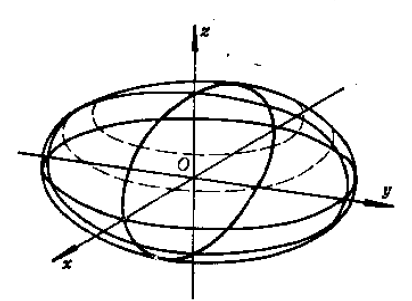
\includegraphics[width=0.36\textwidth]{pic/ga-1012/ga-1012-1.png}
\caption{\text{椭球面}}
\end{figure}
\begin{enumerate}
\item 伸缩法
由单位球面
\[
x^2+y^2+z^2=1
\]
沿 $x,y,z$ 轴分别拉伸 $a,b,c$ 倍，得到椭球面
\[
\frac{x^2}{a^2}+\frac{y^2}{b^2}+\frac{z^2}{c^2}=1.
\]
\item 截痕法
用$z=h$去截,得椭圆
\(\left \{ \begin{array}{l}
\frac{x^2}{a^2}+\frac{y^2}{b^2} = 1 - \frac{h^2}{c^2} \\
z = h
\end{array} \right .\)
其顶点为$( \pm a \sqrt{1-\frac{h^2}{c^2}} , 0 , h)$及$(0 ,  \pm b \sqrt{1-\frac{h^2}{c^2}} , h)$
当 $h$ 变化时，顶点轨迹为
\(\left\{
\begin{array}{l}
\frac{x^2}{a^2}+\frac{z^2}{c^2}=1,\\
y=0
\end{array}
\right.\)
及
\(\left\{
\begin{array}{l}
\frac{y^2}{b^2}+\frac{z^2}{c^2}=1,\\
x=0
\end{array}
\right.\)
它们是一对正交的,有公共顶点的椭圆
椭球面可以看作是一个椭圆(动)变化得到的,变化中保持顶点在上述椭圆对(静),且始终垂直于它们公共的顶点的连线
\end{enumerate}

\subsection*{2. 单叶双曲面}

\[
\frac{x^2}{a^2}+\frac{y^2}{b^2}-\frac{z^2}{c^2} = 1
\]
\begin{figure}[htbp]
\centering
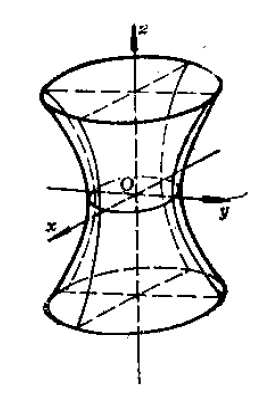
\includegraphics[width=0.36\textwidth]{pic/ga-1012/ga-1012-2.png}
\caption{\text{单叶双曲面}}
\end{figure}
\begin{enumerate}
\item 伸缩法
由双曲线
\[
\left\{
\begin{array}{l}
\frac{y^2}{b^2}-\frac{z^2}{c^2}=1,\\
x=0
\end{array}
\right.
\]
绕 $z$ 轴（双曲线的虚轴）旋转，得到
\[
\frac{x^2+y^2}{b^2}-\frac{z^2}{c^2}=1.
\]
再沿 $x$ 轴拉伸 $\dfrac{a}{b}$ 倍，得到原曲面。
\item 截痕法
用$z = h$去截,得到椭圆
\(\left \{ \begin{array}{l}
\frac{x^2}{a^2}+\frac{y^2}{b^2} = 1 + \frac{h^2}{c^2} \\
z = h
\end{array} \right .\)
其顶点为$( \pm a \sqrt{1+\frac{h^2}{c^2}} , 0 , h)$及$(0 ,  \pm b \sqrt{1+\frac{h^2}{c^2}} , h)$
当 $h$ 变化时，顶点轨迹为
\(\left\{
\begin{array}{l}
\frac{x^2}{a^2}-\frac{z^2}{c^2}=1,\\
y=0
\end{array}
\right.\)
及
\(\left\{
\begin{array}{l}
\frac{y^2}{b^2}-\frac{z^2}{c^2}=1,\\
x=0
\end{array}
\right.\)
它们是一对正交的,有公共虚轴及虚轴长的双曲线
单叶双曲面可以看作是椭圆(动)变化得到,变化中保持顶点在上述双曲线对(静)上,且垂直于它们的公共虚轴
\end{enumerate}

\subsection*{3. 双叶双曲面}

\[
\frac{x^2}{a^2}-\frac{y^2}{b^2}-\frac{z^2}{c^2} = 1
\]
\begin{figure}[htbp]
\centering
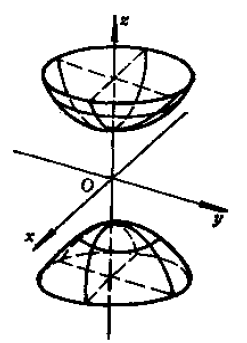
\includegraphics[width=0.36\textwidth]{pic/ga-1012/ga-1012-3.png}
\caption{\text{双叶双曲面}}
\end{figure}
\begin{enumerate}
\item 旋转法
由双曲线
\[
\left\{
\begin{array}{l}
\frac{x^2}{a^2}-\frac{y^2}{b^2}=1,\\
z=0
\end{array}
\right.
\]
绕 $x$ 轴旋转得到
\[
\frac{x^2}{a^2}-\frac{y^2+z^2}{b^2}=1.
\]
再沿 $z$ 轴方向拉伸 $\dfrac{c}{b}$ 倍，得到原曲面。
\item 截痕法
用$x = h$去截,得到椭圆
\(\left \{ \begin{array}{l}
\frac{y^2}{b^2}+\frac{z^2}{c^2} = \frac{h^2}{a^2} - 1 \\
x = h
\end{array} \right .\)
其顶点为$(h,  \pm b \sqrt{\frac{h^2}{a^2}-1} , 0)$及$(h , 0 ,  \pm c \sqrt{\frac{h^2}{a^2}-1})$
当 $h$ 变化时，轨迹为
\(\left\{
\begin{array}{l}
\frac{x^2}{a^2}-\frac{y^2}{b^2}=1,\\
z=0
\end{array}
\right.\)
及
\(\left\{
\begin{array}{l}
\frac{x^2}{a^2}-\frac{z^2}{c^2}=1,\\
y=0
\end{array}
\right.\)
它们是一对正交的,且有公共的实轴及实轴长的双曲线
双叶双曲面可以看作是椭圆(动)变化得到,变化中保持顶点在上述双曲线对(静)上,且垂直于它们的公共实轴
\end{enumerate}

\subsection*{4. 椭圆抛物面}

\[
z = \frac{x^2}{a^2} + \frac{y^2}{b^2}
\]
\begin{figure}[htbp]
\centering
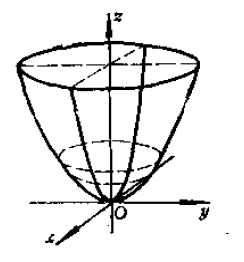
\includegraphics[width=0.36\textwidth]{pic/ga-1012/ga-1012-4.png}
\caption{\text{椭圆抛物面}}
\end{figure}
\begin{enumerate}
\item 旋转法
由抛物线
\[
\left\{
\begin{array}{l}
z=\frac{x^2}{a^2},\\
y=0
\end{array}
\right.
\]
绕 $z$ 轴旋转，得到旋转抛物面
\[
z=\frac{x^2+y^2}{a^2}.
\]
再沿 $y$ 轴拉伸 $\dfrac{b}{a}$ 倍，得到原曲面。
\item 截痕法
用$z = h$去截,得到椭圆
\(\left \{ \begin{array}{l}
\frac{x^2}{a^2}+\frac{y^2}{b^2}=h,\qquad z=h
\end{array} \right .\)
其顶点为 $(\pm a\sqrt{h},0,h)$ 和
$(0,\pm b\sqrt{h},h)$。
当 $h$ 变化时，轨迹为
\(\left\{
\begin{array}{l}
z=\frac{x^2}{a^2},\\
y=0
\end{array}
\right.\)
和
\(\left\{
\begin{array}{l}
z=\frac{y^2}{b^2},\\
x=0
\end{array}
\right.\)
它们是一对正交的,有公共对称轴,公共开口方向及顶点的抛物线
椭圆抛物面可以看作椭圆(动)变化得到,变化中保持顶点在上述抛物线对(静)上,且和公共的对称轴垂直
\end{enumerate}

\subsection*{5. 双曲抛物面(马鞍面)}

\[
z = \frac{x^2}{a^2} - \frac{y^2}{b^2}
\]
\begin{figure}[htbp]
\centering
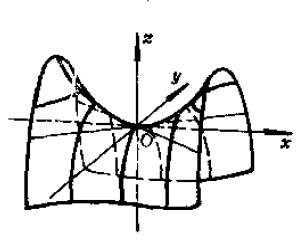
\includegraphics[width=0.36\textwidth]{pic/ga-1012/ga-1012-5.png}
\caption{\text{双曲抛物面}}
\end{figure}
截痕法
用$x = h$去截,得到抛物线
\[
\left\{
\begin{array}{l}
z=\frac{h^2}{a^2}-\frac{y^2}{b^2},\\
x=h
\end{array}
\right.
\]
其对称轴为 $z$ 轴，开口方向为 $z$ 轴负方向，
顶点为 $\left(h,0,\frac{h^2}{a^2}\right)$，开口大小与 $h$ 无关。
顶点的轨迹也是一个抛物线
\[
\left\{
\begin{array}{l}
z=\frac{x^2}{a^2},\\
y=0
\end{array}
\right.
\]
对称轴z轴,顶点为$(0,0,0)$,开口方向为z轴
取抛物线
\[
\left\{
\begin{array}{l}
z=-\frac{y^2}{b^2},\\
x=0
\end{array}
\right.
\]
（动），双曲抛物面可以看作是一对抛物线：它们正交，有公共的对称轴，开口方向相反且有公共的顶点，其中一条的顶点沿着另外一条平行移动所得到的图形。

\subsection*{二次曲线}

\[
a_{11}x^2+2a_{12}xy+a_{22}y^2+2b_1x+2b_2y+c=0
\]
\begin{enumerate}
\item 消去交叉项
设旋转前后的单位基向量分别为
$\vec e_1,\vec e_2$ 和 $\vec e_1',\vec e_2'$，则
\[
\left\{
\begin{array}{l}
\vec e_1'=\cos\theta\,\vec e_1+\sin\theta\,\vec e_2,\\
\vec e_2'=-\sin\theta\,\vec e_1+\cos\theta\,\vec e_2.
\end{array}
\right.
\]
对应的坐标变换为
\[
\left\{
\begin{array}{l}
x=\cos\theta\,x'-\sin\theta\,y',\\
y=\sin\theta\,x'+\cos\theta\,y'
\end{array}
\right.
\qquad\text{（坐标变换公式）}
\]
将坐标变换代入二次项
$a_{11}x^2+2a_{12}xy+a_{22}y^2$，其中 $x'y'$ 的系数为
\[
a_{11}(-2\sin\theta\cos\theta)
{}+2a_{12}(\cos^2\theta-\sin^2\theta)
{}+a_{22}(2\sin\theta\cos\theta).
\]
令该系数为 $0$，得到
\[
\cot{2 \theta} = \frac{a_{11} - a_{22}}{2a_{12}}
\]
例
\[
x^2-xy+y^2+2x+y-1 = 0
\]
先旋转,计算$\theta = \frac {\pi}{4}$
得
\[
\frac{1}{2}x'^2+\frac{3}{2}y'^2
+\frac{3\sqrt{2}}{2}x'
-\frac{\sqrt{2}}{2}y'-1=0.
\]
再平移有
\[
\frac{1}{2}\left(x'+\frac{3\sqrt{2}}{2}\right)^2
+\frac{3}{2}\left(y'-\frac{\sqrt{2}}{6}\right)^2
=\frac{10}{3}.
\]

\end{enumerate}
\end{document}
